% TO:DO
% Add David cell example as motivational example to Introduction to help explain levels of concepts
%
% Use haskell syntax for haskell code examples
%
% Update examples (such as figure 1) to use David cell too
% 
% Create one big figure to show the design flow in Workcraft
% 
% In "Using Plato from Workcraft" section, remove things that could be outdated due to future implementations
%
% Remove some references, some are old, some have been updated
% 
% Generally ensure that the whole paper runs smoothly, everything is in order, and nothing referes to an old version of this paper
%


\documentclass[british,conference,compsoc]{IEEEtran}
\usepackage[T1]{fontenc}
\usepackage{float}
\usepackage{amsmath}
\usepackage{amssymb}
\usepackage{graphicx}
\usepackage{setspace}
\usepackage{array}
\usepackage{blindtext}
\usepackage{listings}

\makeatletter

\newcommand{\noun}[1]{\textsc{#1}}

\@ifundefined{showcaptionsetup}{}{
 \PassOptionsToPackage{caption=false}{subfig}}
\usepackage{subfig}
\makeatother

\usepackage{babel}
\usepackage{algpseudocode}
\usepackage{algorithm}

\begin{document}

\twocolumn

\title{Plato: a tool for behavioural 
\\ specification of asynchronous circuits}
\author{Jonathan Beaumont\\
\texttt{j.r.beaumont@ncl.ac.uk}\\
\emph{School of Electrical and Electronic Engineering, Newcastle University,
UK}}

\maketitle

\begin{abstract}
Asynchronous circuits are becoming increasingly important in
system design, where they orchestrate
the interface between synchronous computation components
and the analogue environment.
However, wide adoption of asynchronous circuits by industrial users is
hindered by a steep learning curve for asynchronous control models,
such as Signal Transition Graphs, that are developed by the academic
community for specification, verification and synthesis of
asynchronous circuits.

Previously, we have introduced a novel high-level description language
for asynchronous circuits, which is based on behavioural
\textit{concepts} -- high-level descriptions of asynchronous circuit
requirements.
In this paper we will discuss our open-source tool, \noun{Plato} 
which allows the specification of asynchronous circuits using concepts, and 
features the ability to automatically translate these to Signal Transition 
Graphs for further processing by conventional asynchronous EDA 
tools, such as \noun{Petrify} and \noun{Mpsat}.
\end{abstract}

\sloppy
\thispagestyle{empty}

\vspace{-3mm}

\section{Introduction}

\vspace{-3mm}

\emph{Concepts} have been presented in order to provide a more compact, 
adaptive and intuitive method of designing asynchronous circuits, using a fully
compositional description method. This was born out of the use of algebra for 
designing systems, such as the model Conditional Partial Order
Graphs~\cite{CPOG1}\cite{CPOG2}\cite{2014_mokhov_pg} and
the algebra of switching networks~\cite{mokhov2015algebra}. Composition is an 
important part of concepts and the use of composition in some algebraic 
representations, such as with DI algebra~\cite{270632} and Conditional Signal 
Graphs~\cite{6243877} helped to inspire this. 

As discussed in~\cite{2015_Beaumont_MEMOCODE}, concepts are a useful language 
for specifying the behaviours of asynchronous circuits, in the preferred form 
of the user. This can be as low-level signal-level concepts, or higher-level 
gate- or protocol-level concepts. It also allows the definition of their own 
concepts, which can be reused within the same or any other specification that 
they wish to increase the speed of designing a system, and future systems. 

With concepts, we aim to solve the problems that can arise from the more 
commonly used monolithic approach, where a user must design each system in the 
form of an STG from a blank page. The scalability of this is poor: as the 
system grows in complexity its monolithic specification becomes challenging to 
comprehend and debug. The problem becomes particularly severe when designing 
multi-mode systems, such as power regulators, where capturing all aspects of 
system behaviour in a consistent specification is a major design 
challenge~\cite{2014_sokolov_ftfc}\cite{sokolov2015design}. 
Moreover, the STG models of components and operating modes are difficult to 
reuse when designing other specifications, and thus each new design must be 
built from the ground up. This is particularly undesirable for industry, as 
this increases the design time of each design greatly. 

STGs~\cite{Chu_1987_phd}\cite{Rosenblum_1985_tpn} are commonly used for the 
specification, verification and synthesis of asynchronous control circuits as 
they are supported by multiple EDA tools, such as 
\noun{Petrify}~\cite{Cortadella}, \noun{Mpsat}~\cite{khomenko2004detecting}, 
\noun{Versify}~\cite{i1997formal}, 
\noun{Workcraft}~\cite{2007_poliakov_workcraft}\cite{Workcraft_website}, 
and others.

These tools take an STG specification and can formally verify its correctness, 
as well as synthesise an asynchronous circuit implementation that is \
emph{speed-independent}, i.e. guaranteed to work correctly regardless of 
component delays~\cite{Muller_1959_ts}.

Concepts are not supported by these tools, and rather than
authoring tools to verify and synthesize concepts directly, which is a time 
consuming process, we can \emph{translate} concepts to STGs, for use with these
existing tools.

In this paper, we will discuss the implementation of the domain specific 
language and translation tool for concepts, called 
\noun{Plato}~\cite{2016_concepts_github} embedded in Haskell. 
If STGs are the assembly language of asynchronous circuits, \noun{Plato} is a 
compiler from a higher-level language, concepts, to this assembler. 

\noun{Plato} is 
integrated into \noun{Workcraft}~\cite{Workcraft_website}, an open-source 
EDA tool which also features some verification and synthesis tools for STGs, 
and we will discuss the use of the tool from within \noun{Workcraft}.

The contributions of this paper are:
\vspace{-1mm}
\begin{itemize}
  \item We detail the notations of concepts within \noun{Plato} and the built in
  concepts and their uses in Section~\ref{sec:tool-func}
  \item We explain how to use the tool both stand-alone and within
  \noun{Workcraft} to translate concepts in Section~\ref{sec:tool-use}.
  \item We present the implemented algorithm for translating concepts to STGs
  in Section~\ref{sec:algorithm}.
\end{itemize}

\section{Features of \noun{Plato}\label{sec:tool-func}}

\vspace{-3mm}

The abstract base of concepts, on which these asynchronous specificications of 
circuits is discussed in~\cite{2015_Beaumont_MEMOCODE}.

\vspace{-3mm}

\subsection{Concept notation \label{sub:concept-notation}}

\vspace{-3mm}

Concepts can be composed of other concepts, and this applies to the behaviours 
of signals, as well as the specifying of the initial states and the signal 
types. This allows there to be different levels of concepts, each level of 
which will feature a composition of concepts from a lower level. 

In this section we will explain these levels, and the standard notations of 
concepts for these. 

\vspace{-2mm}

\subsubsection{\label{signal-level}Signal-level concepts}Asynchronous circuit 
specifications are mainly composed of signal transitions, and interactions 
between these, to show causal relationships. Signal transitions are denoted as 
$a^{+}$ and $a^{-}$, where $a$ is any signal name, at least one character, and 
the $+$ or $-$ indicates which way the this signal transitions, $+$ denoting a 
low-to-high or 0 to 1 transition, and $-$ denoting a high-to-low, 1 to 0 
transition. 

\noun{Plato} is written in Haskell, a functional programming language. The 
domain specific language which we have implemented therefore uses Haskell 
notations, and this means some notations are different to standard signal 
transition specifications. $a^{+}$ and $a^{-}$ are in post-fix notation, where 
the operator is stated after the operand. Haskell does not support post-fix 
notation, and as such, we have to use a differing signal transition notation. 

For the tool, signal transitions $a^{+}$ and $a^{-}$ are noted as $rise\,a$ and 
$fall\,a$ respectively. We will use the tool notation for examples, but 
describe these using standard notation.

Signal-level concepts are the base level of concepts, and are 
the type all other concepts are built on. Here we display the standard concepts
available at this level.

A key concept in asynchronous circuits is \emph{causality}:
one signal transition \emph{causes} another signal transition, a cause and an 
effect. This is denoted in the form: 

\vspace{-3mm}

\[
rise\,a \sim> rise\,c
\]

\vspace{-1mm}

This is read as $a^{+}$ causes $c^{+}$, meaning that for the $c^{+}$ transition 
to occur, $a^{+}$ must have occurred previously. The $\sim>$ 
operator is used to show causal relationships between signals.
 
While this concept is called \emph{causality}, this doesn't necessarily imply
timings, such as any $\mathit{cause}$ transition immediately forcing the
 $\mathit{effect}$ transition it applies to. Causality can be used in order to
list all possible $\mathit{cause}$ transitions which need to occur in order
 for an $\mathit{effect}$ transition.

One can compose any concepts using the $<>$ (diamond) operator, and this applies
to concepts of any level, whether predefined or user-defined. For example, 
two causality concepts can be composed.

\vspace{-3mm}

\[
rise\,a\sim> rise\,c\ <> \ rise\,b\sim> rise\,c
\]

\vspace{-1mm}

In words, $a^{+}$ \emph{and} $b^{+}$ must occur before $c^{+}$ can occur. 
This corresponds to so-called AND-causality in the fact that several cause 
transitions \emph{must all} have occurred before an event can occur. 
AND-causality is commonly used to imply behaviours in circuits, for specific 
requirements of effect transitions.  

The above notation can cause long-winded specifications when lots of 
AND-causality is involved. To solve this we provise a listing option. The 
following will acheive the same results:

\vspace{-3mm}

\[
[rise\,a, rise\,b]\sim\hspace{-1.5mm}\&\hspace{-1.5mm}\sim\hspace{-1.5mm}>rise\,c
\]

\vspace{-1mm}

This form of concept can be composed as usual with any other concepts.

A less common, but still useful form of causality is OR-causality. This is 
where an effect transition can have several possible cause transitions. Only 
one cause transition is required to occur to allow the effect transition to 
occur. 

With OR-causality, the notation used lists all possible causes for the stated 
effect:

\vspace{-2mm}

\[
[rise\,x, rise\,y]\sim\hspace{-1.5mm}|\hspace{-1.5mm}\sim\hspace{-1.5mm}>rise\,z
\]

\vspace{-1mm}

This is, \emph{either} $x^{+}$ \emph{or} $y^{+}$ must occur in order for 
$z^{+}$ to occur.

The interactions when an effect transition is included in both AND- and 
OR-causality are interesting, and an example of when this occurs can be found 
in Section~\ref{sec:algorithm}.

\vspace{-2mm}

\subsubsection{Gate-level concepts} Using the causality concept we can express
the behaviour of gates in asynchronous circuits. For example, a \emph{buffer}
is a gate with one input signal and one output signal,
whose output transitions causally depend on the input ones:

\vspace{-4mm}

\[
\mathsf{buffer}\,a\,b=rise\,a \sim> rise\,b\ <>\
fall\,a\sim> fall\,b
\]

\vspace{-1mm}

\noindent An \emph{inverter} has a similar conceptual specification, but the
output transition is inverted:

\vspace{-4mm}

\[
\mathsf{inverter}\,a\,b=rise\,a\sim> fall\,b\ <>\
fall\,a\sim> rise\,b
\]

\vspace{-1mm}

\noindent A \emph{C-element} is a gate with two inputs, in this example $a$ and $b$, and one
output~$c$, which synchronises both rising and falling input transitions
via AND-causality:

\vspace{-3mm}

\[
\begin{array}{lcl}
\mathsf{cElement}\,a\, b\, c=&\hspace{-9mm}rise\,a\!\sim>\! 
	rise\,c\ <> rise\,b\!\sim>\! rise\,c\ \\
&\hspace{-5mm}<>\hspace{-1mm} fall\,a\!\sim>\! fall\,c\ \,
	<>\ fall\,b\!\sim>\! fall\,c
\end{array}
\]

\vspace{-1mm}

An alternative way to express the same concept is to reuse the buffer concept:

\vspace{-3mm}

\[
\mathsf{cElement}\,a\, b\, c=\mathsf{buffer}\,a\, c <> \mathsf{buffer}\,b\, c
\]

\vspace{-1mm}

A C-element combines the constraints imposed on the output
transitions by two `virtual' buffers. Behaviour of other gates can be similarly
defined in this way. An expanded example of a C-element and other examples can 
be found in~\cite{2015_Beaumont_MEMOCODE}.

\vspace{-2mm}

\subsubsection{Protocol-level concepts} In addition to gate-level concepts
described above it is often important to specify \emph{protocols}
of interaction between multiple gates, components or signals. 

Here we demonstrate how one can use concepts to specify asynchronous handshakes
and mutual exclusion mechanisms.

Given two signals $a$ and $b$, a \emph{handshake} between them is
the following composition of causality concepts:

\[
\begin{array}{lcl}
\mathsf{handshake}\,a\, b=&\hspace{-7mm}rise\,a\!\sim>\! rise\,b\ 
	<>\ rise\,b\!\sim>\! fall\,a \\
&\hspace{-5mm}<>\hspace{-1mm} fall\,a\!\sim>\! fall\,b \, 
	<>\ fall\,b \sim>\! rise\,a
\end{array}
\]

Intuitively, we have a two-way asynchronous communication channel,
where one party sends transitions $a^{+}$ and $a^{-}$ and the other
party responds by corresponding $b^{+}$ and $b^{-}$ transitions.
Note that the four causality concepts match those found
in the buffer and inverter concepts, which leads to an alternative
way to express a handshake between~$a$ and~$b$:

\vspace{-3mm}

\[
\mathsf{handshake}\,a\, b=\mathsf{buffer}\,a\, b <>\mathsf{inverter}\,b\, a
\]

\vspace{-1mm}

This conceptual understanding of a handshake as being composed
from a buffer and an inverter is often used by circuit designers as
a convenient way of reasoning.

\vspace{-2mm}

\subsection{Concepts required for translation\label{sub:trans-concepts}}

\vspace{-2mm}

The concepts we have discussed so far are aimed at specifying the behaviour of 
signals in a circuit. When translating these to STGs however, these behaviours 
do not necessarily result in a correct specification, meaning they will not be 
verifiable by standard tools, and therefore not useful in further operations, 
such as synthesis.

This is due to various parts of an STG that we have not yet discussed, which 
are important for specification, namely \emph{interface} and 
\emph{initial states}.

\vspace{-3mm}

\subsubsection{Interface concepts\label{sub:interface}} 

An important part of a specification is how these signals interact with the 
outside world, which could be another scenario or another circuit, for example.
These signals can be inputs from the outside world, outputs or an internal 
signal, which is used only within this scenario. 

To specify the type of a signal (\emph{input},
\emph{output} or \emph{internal}) we introduce the \textsf{interface} concept.
Signal types are composed according to the following rules:

\vspace{-2mm}

\[
\begin{array}{|l||l|l|l|}
\hline
\multicolumn{1}{|c||}{<>} & \mathsf{Input} & \mathsf{Output} &
\mathsf{Internal} \\ \hline \hline
\mathsf{Input} & \mathsf{Input} & \mathsf{Output} & \mathsf{Internal} \\ \hline
\mathsf{Output} & \mathsf{Output} & \mathsf{Output} & \mathsf{Internal} \\
\hline
\mathsf{Internal}& \mathsf{Internal} & \mathsf{Internal} & \mathsf{Internal} \\
\hline
\end{array}
\]

The intuition is as follows:
\begin{itemize}
    \item If a signal is an input in one component of the system, but is an
    output in another components, then in the composition it will be an output.
    \item An internal signal is similar to an output signal in the sense
that it is driven by the circuit (not the environment), but it is hidden, 
i.e.not accessible via the circuit interface. Once a signal is hidden and 
declared internal it cannot be revealed.
\end{itemize}

\noindent Specifying signal types is important when designing asynchronous
circuits, as it helps to quickly identify errors (e.g. an input transition is
caused by a hidden internal transition), and reuse existing tools for circuit
simulation, verification and synthesis. Signal type information is also used
in the algorithm for automated translation of concepts to
STGs (Section~\ref{sec:algorithm}).

Concepts \textsf{inputs}, \textsf{outputs}, \textsf{internals} are defined for
specifying types of sets of signals for convenience, and to be included inline 
with other concepts. For example, to specify that signals $a$ and $b$ are 
inputs, $c$ is an output, and $t$ is internal, it is possible to write:

\vspace{-4mm}

\[
\mathsf{inputs}\,[a, b] <> \mathsf{outputs}\,[c] <>
\mathsf{internals}\,[t].
\]

\vspace{-4mm}

\subsubsection{Initial state concepts\label{sub:initState}}

Specifying the initial state is important, as it determines what the first 
transitions of a scenario will be. Without these, no transition can occur.

Each signal must have it's initial state declared before translation can occur. 
In order to specify the initial state of a handshake between signals~$a$
and~$b$, we use the $\mathsf{initialise}$ concept.
The possible initial states are \emph{high} or \emph{low}, referred to as 
\emph{0} or \emph{1} respectively:

\vspace{-2mm}

\[
\mathsf{initialise}\,a\,0 <> \mathsf{initialise}\,x\, 1
\]

\vspace{-1mm}

\noindent A signal can only be declared as initially high or low. If the 
initial state of a signal is not defined, an error will occur, and the 
translation will not continue. Conversely, if the event a signal has it's 
initial state declared as both high and low, and is thus inconsistent, in a 
specification then the translation will also fail.

For the ease of use, and to speed up the process, initial states can also be 
declared in lists by on state:

\vspace{-2mm}

\[
\mathsf{initialise0}\, [a, b, c] <> \mathsf{initialise1}\, [x, y]
\]

\vspace{-1mm}

\noindent As an example, we can include this in the specification of a 
handshake, to create a handshake with built-in initial state.
$\mathsf{initialise}\,a\, 0$ sets the state of the signal
$a$ to $0$. We can compose an initial state concept with the handshake concept
into a combined $\mathsf{handshake00}\,a\, b$ concept as

\vspace{-3mm}

\[
\begin{array}{lcl}
\mathsf{handshake00}\, a\, b =&\hspace{-2mm}\mathsf{handshake}\,a\, b 
	<> \mathsf{initialise}\,a\, 0 \\
&\hspace{-6mm}<> \mathsf{initialise}\,b\, 0
\end{array}
\]

\vspace{-1mm}

The resulting concept corresponds to a handshake between signals~$a$
and~$b$ that are both initially $0$.

\vspace{-2mm}

%\subsection{Built-in concepts\label{sub:built-in}}
%
%\vspace{-3mm}
%
%In our previous paper, \cite{2015_Beaumont_MEMOCODE}, we have displayed several
%examples of different concepts and how they can be described in terms of 
%concepts in several ways, either from base level signal-level concepts, or 
%through reuse of pre-defined gate- and protocol-level concepts.
%
%In this section, we will detail further concepts included with the \noun{Plato}
%along with those already described in Sections~\ref{sub:concept-notation} 
%and~\ref{sub:trans-concepts}. All of these are often used in the specification 
%of asynchronous circuits and therefore it is useful to include them, to avoid a 
%user having to define these for each specification. For each of these we will 
%explain their use for asynchronous circuits, and give the standard usage of the 
%concept. 
%
%\begin{itemize}
%  
%  \item $\mathsf{handshake11}\,a \,b$ is a protocol-level concept, similar to 
%  $\mathsf{handshake00}\,a \,b$ as discussed in Section~\ref{sub:initState}. 
%  The behaviours of the signals are the same as in the standard 
%  \texttt{handshake} concepts, but this includes initial states for the 
%   signals. For this concept, both signals will be initialised to 1, or high.
%\vspace{-4mm}  
%  \item []
%  
%  \item $\mathsf{me}\,a \,b$ is a protocol-level concept. This concept defines 
%  \emph{Mutual Exclusion} between two signals. This means that when one 
%  of these signals is high, the other cannot transition high.
%\vspace{-4mm}
%  \item []
%  
%  \item $\mathsf{meElement}\,r1\,r2\,g1\,g2$ is a gate-level concept to 
%  apply the mutual exclusion protocol. In this case, there are four signals. 
%  Two are intputs ($r1$ and $r2$), the other two are 
%  outputs~($g1$ and $g2$). $r1$ transitioning high will cause $g1$ to go
%  transition high, and this is the same for $r2$ and $g2$, however,
%  $g1$ and $g2$ are mutually exclusive. The aim of this concept is to 
%  ensure that the request signals, $r1$ and $r2$, cause their respective
%  grant signals, $g1$ and $g2$, to transition high but never at the same 
%  time. 
%\vspace{-4mm}
%  \item []
%  
%  \item $\mathsf{andGate}\,a\,b\,c$ is a gate-level concept, using 
%  OR-causality to implement a standard AND gate. Signals $a$ and 
%  $b$ are inputs to the gate, and $c$ is the output. \emph{Both} 
%  $rise a$ \emph{and} $rise b$ must occur for $rise c$ to occur. 
%  Following this, \emph{either} $fall a$ \emph{or} $fall b$ must 
%  occur for $fall c$ to occur.
%\vspace{-4mm}
%  \item []  
%
%  \item $\mathsf{orGate}\,a\,b\,c$ is a gate-level concept, also using 
%  OR-causality. Signals $a$ and $b$ are inputs to the gate, and $c$ is the 
%  output. \emph{Either} $rise a$ \emph{or} $rise b$ must occur for $rise c$ to 
%  occur. Following this, \emph{both} $fall a$ and $fall b$ must occur for 
%  $fall c$ to occur. 
%  
%\end{itemize}
%
%\noindent All of the concepts described in this section are some of the most
%common behaviours found in asynchronous circuits, and these can be used
%to specify many different asynchronous circuits. 
%
%These can also be used in order to define new protocols and gates for a designer
%to use in their own specifications, making the design process easier in future 
%systems. 
%
%\vspace{-3mm}

\section{Concepts to STG translation algorithm\label{sec:algorithm}}

\vspace{-2mm}

Concepts are a useful way of specifying asynchronous circuits, but
specifications also need to be \emph{verified} against certain properties to
ensure their correctness, and once they are deemed to be correct, they need to
be \emph{synthesised} into efficient circuit implementations. Many software
tools exist which automatically verify and synthesise STG specifications,
such as \noun{Petrify}~\cite{Cortadella} and
\noun{Mpsat}~\cite{khomenko2004detecting}.

In order to reuse the tools developed by the community, it is
necessary to be able to automatically translate concept specifications to STGs.
In this section, we will display an example of how the translation algorithm 
operates, and present a pseudocode form of the algorithm in 
Algorithm~\ref{alg:translation}. 

We will use the OR-gate example, the specification of which can be seen in 
Section~\ref{sub:file_layout}. This is a rudimentary example, but is useful in 
displaying how the algorithm handles a system featuring both OR- and 
AND-causality.

There are multiple ways of representing a specification using concepts. However,
all levels of abstraction available to the designer are built out of primitive 
low-level signal concepts. Given a specification, we can therefore break down 
all gate- and protocol-level constructs into `atoms', which significantly 
simplifies the translation task.

For this example, the specification is broken down into these signal-level 
concepts:

\vspace{-4mm}
\[
\begin{array}{lcl}
\hspace{-2mm}\mathsf{circuit}\,a,\,b,\,c&\hspace{-2mm}=
	&\hspace{-2mm}[a^{+}, b^{+}]
	\sim\hspace{-1.5mm}|\hspace{-1.5mm}\sim\hspace{-1.5mm}>c^{+}\\
~&\hspace{-2mm}&<>a^{-}\sim> c^{-} <> b^{-}\sim> c^{-}\\
~&\hspace{-2mm}&<> \mathsf{inputs} \, [a,\,b] <>\mathsf{outputs}\,[c] \\
~&\hspace{-2mm}&<>\mathsf{initialise0}\,[a,\,b,\,c]
\end{array}
\]

\vspace{-1mm}

\noindent The first step is to prepare the read-arcs, and this is done by
reformating these concepts into lists of causes for effects.
Each list will be of possible causes for each OR- and AND-causality signal-level
concept in the specification, meaning that for each OR-causality concept, 
there will be 2 or more signals in the list, and for each AND-causality 
concept there will be a single item list.

For example, taking the concept\\$[a^{+}, b^{+}]
\sim\hspace{-1.5mm}|\hspace{-1.5mm}\sim\hspace{-1.5mm}>c^{+}$, there are
two possible transitions for $c^{+}$ here, $a^{+}$ and $b^{+}$. These therefore 
form a two item list. 

Another example, using 
$a^{-}\sim> c^{-} <> b^{-}\sim> c^{-}$, there are two
cause transitions for $c^{-}$, namely $a^{-}$ and $b^{-}$. Both of these 
therefore form their own single item list. 

This will mean there may be several different lists for each cause transition. 
Table~\ref{tab:list-of-concepts} contains all of the lists described above.

\vspace{-1mm}

\begin{table}[h]
\caption{Lists of cause transitions by effect transitions
		\label{tab:list-of-concepts}}
  \centering
\begin{tabular}[htb]{| m{2.6cm} | m{2.0cm} |}
  \hline
Causes & \, Effect \\ \hline \hline
$a^{+}$, $b^{+}$ & $c^{+}$ \\ \hline
$a^{-}$ & $c^{-}$ \\ \hline
$b^{-}$ & $c^{-}$ \\ \hline
  \end{tabular}
  \vspace{-1mm}
\end{table}

\noindent From this, we can then combine the lists by effect transition, to 
give us a list of lists. This can be viewed in Table~\ref{tab:list-of-lists}.

\vspace{-1mm}

\begin{table}[h]
\caption{Lists of lists of cause transitions
		\label{tab:list-of-lists}}

  \centering
\begin{tabular}[htb]{| m{2.6cm} | m{2.0cm} |}
  \hline
Causes & \, Effect \\ \hline \hline
[$a^{+}$, $b^{+}$] & $c^{+}$ \\ \hline
[$a^{-}$], [$b^{-}$] & $c^{-}$ \\ \hline

  \end{tabular}
 \vspace{-3mm}
\end{table}

\noindent Note how for the $c^{-}$ transition there is 2 different single item 
lists. Each one is an AND-causality, and why they are each in a separate list
will become apparent in the next step. 

This step is applying the \emph{Cartesian Product} to each of the list of lists
for each effect transition. This will "expand the brackets", combining each
item of each list with every item of every other list, creating a single list 
which provides us with the number of this transition and which arcs to connect
for each transition of each type. For this example, it is fairly simple, $c^{+}$
has one list, and therefore the result of the Cartesian Product is the same as 
this list. $c^{-}$ has two single item lists, and performing the cartesian 
product on this will give us $[a^{-}\,b^{-}]$. 

These newly formed lists provide us with the number of transitions for each 
effect transition. This means there will be two $c^{+}$ transitions, as the list
as the result of the Cartesian product is a list of two items. The first 
$c^{+}$ transition will be caused by $a^{+}$, the second will be caused by 
$b^{+}$. 

For $c^{-}$, there will be only one transition requiring both $a^{-}$ and 
$b^{-}$.

Now, we can list the read-arcs to be connected for each transition of $c$.
This can be viewed in Table~\ref{tab:list-by-transition}.

\begin{table}[h]
\caption{List of all effect transitions and their causes
		\label{tab:list-by-transition}}

  \centering
\begin{tabular}[htb]{| m{2.6cm} | m{2.0cm} |}
  \hline
Causes & \, Effect \\ \hline \hline
$a^{+}$ & $c^{+}(0)$ \\ \hline
$b^{+}$ & $c^{+}(1)$ \\ \hline
$a^{-}$, $b^{-}$ & $c^{-}$ \\ \hline
  \end{tabular}
\vspace{-1mm}
\end{table}

The numbers of the $c^{+}$ transitions are necessary for reference
when definining arcs, for example, $b^{+}$ needs to connect to 
$c^{+}(1)$, not $c^{+}(0)$ or just $c^{+}$ as this can cause 
erroneous arcs to be included. 

For clarity, where there is only one transition, such as with $c^{-}$
we will refer to this simply as $c^{-}$, but this is effectively $c^{-}(0)$.

This concludes the part of the algorithm which defines the arcs
and transitions. Next, the algorithm begins to build the STGs. 

First of all, we need to add places for each signal. These are used to
show whether a signal has transitioned high or low at any point. 
A token in a $0$ place for example shows that that signal has 
transitioned low. We add a $0$ and $1$ place for each signal, 
which for this example gives us $a0$, $a1$, $b0$, $b1$, $c0$ and $c1$.

The interface is defined at the start of the algorithm, by listing them as 
$inputs$, $outputs$ or $internals$, so now we need to include all the 
transitions, and connect these to the places to form consistency loops, to 
ensure that all signals in this system can only transition in one way when this 
signal's previous transition was in the opposite direction. 

This is done by taking each transition, and if it is a $+$ transition, 
connecting the $0$ place for this signal to the transition, then connecting 
this transition to the $1$ place for this signal. Conversely, if it is a $-$ 
transition, we connect the $1$ place for this signal to the transition, and 
connect this transition to the $0$ place.

%\begin{figure}[h]
%\vspace{-4mm}
%\begin{centering}
%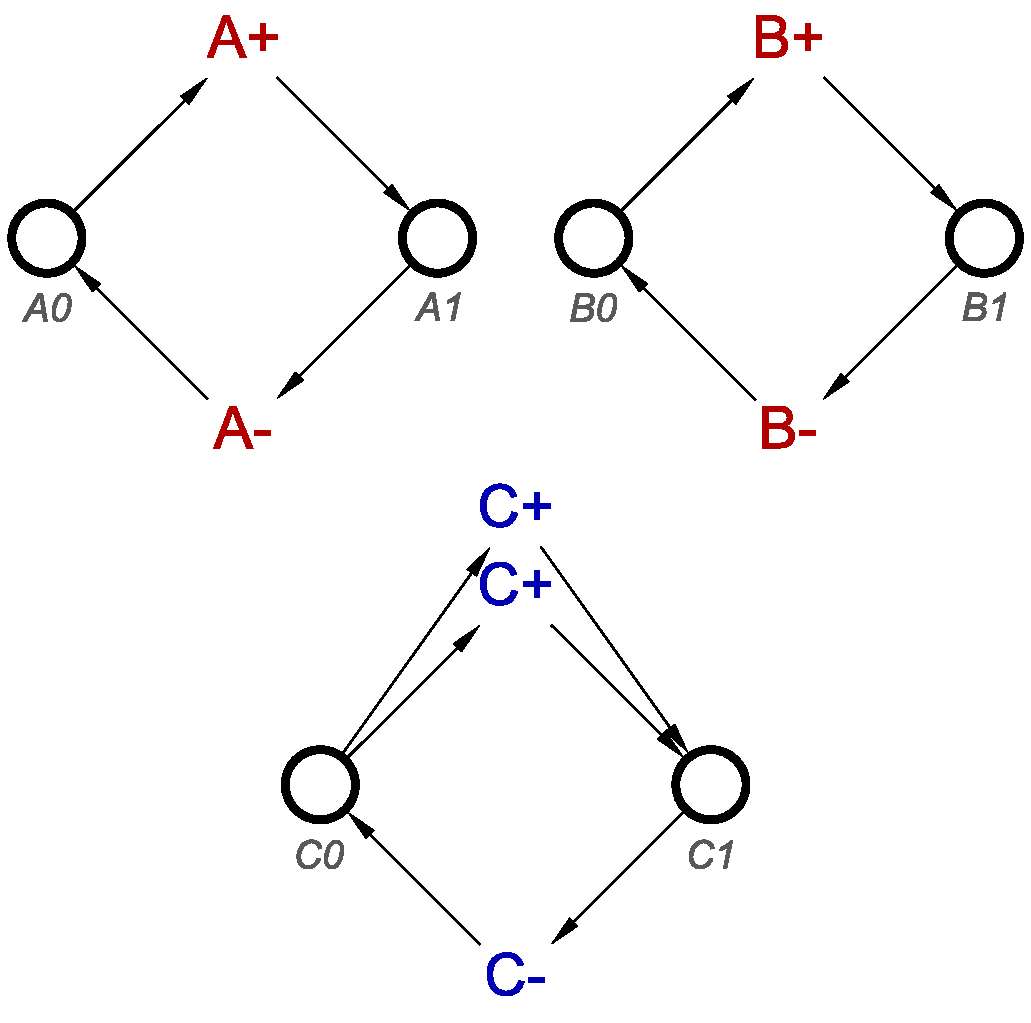
\includegraphics[scale=0.3]{Images/or-gate-loops-stg}
%\par\end{centering}
%%\vspace{-1mm}
%\protect\caption{\label{fig:loops} STG containing only consistency loops}
%\vspace{-1mm}
%\end{figure}

Now the algorithm introduces the initial states. All of the signals are 
specified to be initially 0, meaning that the first transition will be the $+$.
From the consistency loops, to allow this to happen, we need to place a token 
in each $0$ place for each signal. This will produce the STG displayed in 
Figure~\ref{fig:tokens}. Note that both $c^{+}$ transitions are 
included in the consistency loops.

\begin{figure}[h]
\vspace{-4mm}
\begin{centering}
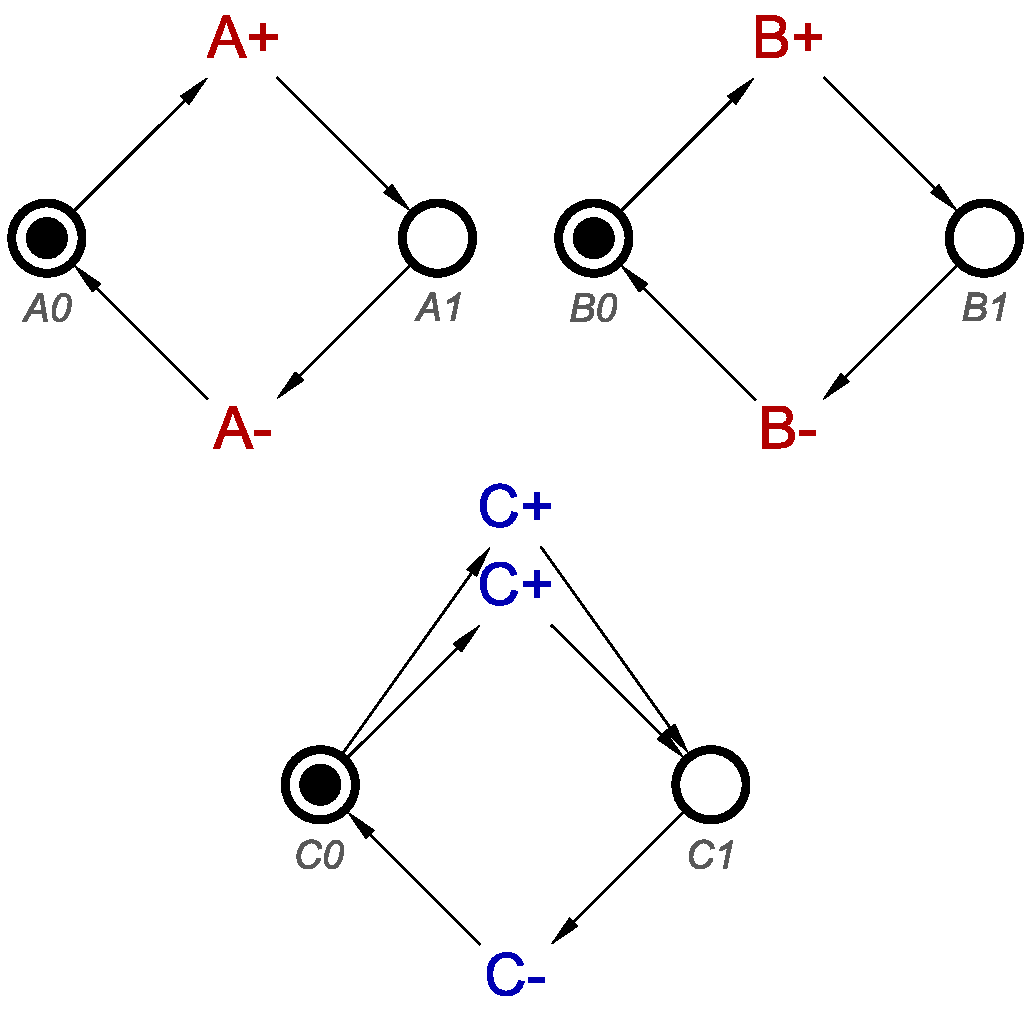
\includegraphics[scale=0.3]{Images/or-gate-inits-stg}
\par\end{centering}
%\vspace{-1mm}
\protect\caption{\label{fig:tokens} STG with consistency loops and 
			initial states}
\vspace{-1mm}
\end{figure}

Finally, we can add the connections to the transitions, and cause the 
expected interaction between signals. We use read-arcs to connect the effect
transitions to the places after the transition of the cause. For example, for
$a^{+} \sim> c^{+}$, we will connect the $a1$ place to the 
transition of $c^{+}$. We use read-arcs for these, as for this example, only
after $c^{+}$ has occured, and placed a token in $x1$, will $c^{+}$ be allowed
to occur, but the read arc will not consume the token in $x1$ which would block
$x^{-}$ from being able to occur. 

Following this, the specification is fully translated, and the resulting STG 
will be the same as shown in Figure~\ref{fig:or-gate-stg}.

\begin{figure}[h]
\vspace{-4mm}
\begin{centering}
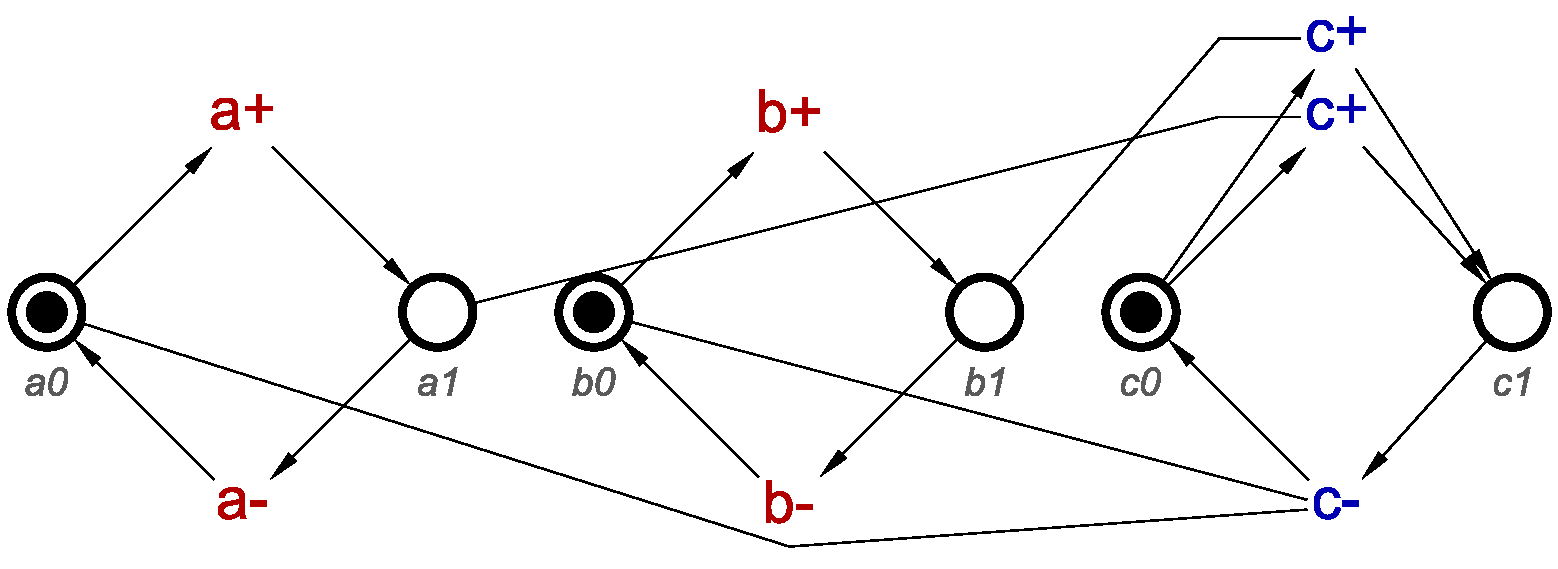
\includegraphics[scale=0.3]{Images/or-gate-stg}
\par\end{centering}
%\vspace{-1mm}
\protect\caption{\label{fig:or-gate-stg} Fully translated OR-gate STG}
\vspace{-5mm}
\end{figure}


\begin{algorithm}[h]
\begin{algorithmic}
\caption{Algorithm for translating concepts to STGs\label{alg:translation}}
\For {Signal $s$ in \textbf{System}}
  \State \textbf{define} interface of $s$ as \emph{Input/Output/Internal}
\EndFor

\For {Each effect transition $e$}
  \State $allCauses$ $\leftarrow$ Concatinate lists  possible causes for $e$
  \State $transitionList$ $\leftarrow$ \emph{Cartesian Product} \textbf{of} 
	$allCauses$
  \For {$i = 0$ to Length of $transitionList$}
    \State \textbf{add} $e(i)$ to $transitions$
  \EndFor 
\EndFor
\For {Each \textbf{signal} $s$ in system}
  \State \textbf{add} place \textbf{$s$.Name}$0$
  \State \textbf{add} place \textbf{$s$.Name}$1$
\EndFor
\For {Each \textbf{transition} $t$ in $transitions$}
  \If {transition is high}
    \State \textbf{connect} (place $t$.signalName$0$, transition)
    \State \textbf{connect} (transition, place $t$.signalName$1$)
    \For {Each \textbf{cause transition} $c$ for $t$}
      \State \textbf{read-arc} (place $t$.signalName$1$, $c$)
    \EndFor
  \EndIf
  \If {transition is low}
    \State \textbf{connect} (place $t$.signalName$1$, transition)
    \State \textbf{connect} (transition, place $t$.signalName$0$)
    \For {Each \textbf{cause transition} $c$ for $t$}
      \State \textbf{read-arc} (place $t$.signalName$0$, $c$)
    \EndFor
  \EndIf
\EndFor
\For {Each initial state $state$ concept}
  \If {$state$ is low}
    \State \textbf{add-token}(\textbf{signalName.place}$0$)
  \EndIf 
  \If {$state$ is high}
    \State \textbf{add-token}(\textbf{signalName.place}$1$)
  \EndIf
\EndFor
\end{algorithmic}
\end{algorithm}


\section{Usage of the tool\label{sec:tool-use}}

\vspace{-2mm}

%In this section, we will cover how to install the tool, how to prepare a
%concepts file and run \noun{Plato} either through command line, or through 
%\noun{Workcraft}, and the output it produces for each of these cases.

In this section, we will discuss the design flow, including the preparation of 
a concepts file, the translation methods from within \noun{Workcraft}, and 
the uses from the translated STGs. This tool can also be used from command line,
however, the design flow can include a GUI from authoring concepts to synthesis
from within \noun{Workcraft}. 

%\vspace{-2mm}
%
%\subsection{Installing the tool \label{sub:installing}}
%
%\vspace{-2mm}
%
%\noun{Plato} can be downloaded from~\cite{2016_concepts_github} on it's
%own, or it is included in the download of Workcraft. It can be used on 
%\emph{Windows}, \emph{Linux} or \emph{Mac OS X}.
%
%Download either\noun{Plato} or \noun{Workcraft}, extract it and move it to
%a known directory. Using a terminal, navigate to this directory,
%or if using \noun{Workcraft}, navigate to the \noun{Workcraft} directory, and
%then navigate to the \noun{Plato} directory, found in \texttt{tools/concepts} 
%(for \emph{OS X}, the \noun{Workcraft} directory is located within the 
%\texttt{Workcraft.app} contents folder. The concepts tool will be found at 
%\texttt{Contents/Resources/tools/concepts}.
%
%Now, the process of installing the tool is the same, regardless of how you aim 
%to use it. First of all, \noun{stack} needs to be installed 
%(download and instructions available from~\cite{stack_website}. 
%To install stack and \noun{Plato}, run: 
%
%\vspace{-2mm}
%
%\begin{lstlisting}[language=bash]
%  $ stack setup --no-system-ghc
%\end{lstlisting}
%
%\vspace{-1mm}
%
%This will prepare stack to install \noun{Plato}. Now, to build and install
%the tool, simply run:
%
%\vspace{-1mm}
%
%\begin{lstlisting}[language=bash]
%  $ stack build
%\end{lstlisting}
%
%\vspace{-5mm}

\subsection{Concepts file layout \label{sub:file_layout}}

\vspace{-5mm}

\begin{figure}[H]
\begin{centering}

\begin{flushleft}
$\,\mathsf{module}\, Concept \, \mathsf{where}$
\par\end{flushleft}

\begin{flushleft}
$\,\mathsf{import}\, Tuura.Concept.STG$
\par\end{flushleft}

\begin{flushleft}
$\,\mathsf{circuit}\,a \,b \,c=\mathsf{\,interface}\,<> \mathsf{\, operation}
<>\,\mathsf{initialState}$

$\,\,\,\mathsf{where}$
\par\end{flushleft}

\begin{flushleft}
$\,\,\,\,\,\,\mathsf{interface}=\mathsf{inputs}\,[a,b]<>\mathsf{outputs}\,[c]$
\par\end{flushleft}

\begin{flushleft}
$\,\,\,\,\,\,\mathsf{operation}= \mathsf{orGate}\,a\,b\,c$
\par\end{flushleft}

\begin{flushleft}
$\,\,\,\,\,\,\mathsf{initialState}= \, \mathsf{initialise0}\,[a,\,b,\,c]$
\par\end{flushleft}

\par\end{centering}
\vspace{-2mm}
\begin{centering}
\protect\caption{\label{fig:concepts_file}A concepts file}
\vspace{-2mm}
\par\end{centering}

\end{figure}

The concepts file we will discuss is found in Figure~\ref{fig:concepts_file}.
All concept files must be edited in a plain-text editor, and saved with the 
``.hs'' file extension, as the concepts are written in Haskell code. 

The following describes important information about specific lines.

\begin{description}
  \item [Line 1]
  This line must be included in all concept files, as the first line, to 
  identify it as a concepts file.
  
  \item [Line 2] must also remain in all concept files, so that the built-in
  operators and existing gates/protocols can be used. 
  
  \item [Line 3] is where a user can begin to define their concepts. 
  ``\texttt{circuit}'' must begin the line, but after this, a user can choose 
  what characters they wish to represent their signals.
  
  \item [Line 4] is simply ``\texttt{where}''. This is used to separate the main
  concept definition from the user-defined concepts.

\end{description}

\vspace{-1mm}

The lines discussed above are the basics of writing concepts. With this 
information, a user can write concept files, but the following lines can be 
used for ease-of-use, ease-of-understanding, and reuse. 

The example we have used is of that of an OR-gate. We have defined the 
interface, initial state and the operation of this separatley, by defining 
these concepts following the ``'$\mathsf{where}$''. The full circuit 
specification is then composed of all three of these defined concepts. 

%\vspace{-3mm}
%
%\subsection{Using \noun{Plato} from command line}
%
%\vspace{-2mm}
%
%The standard command for the tool is as follows:
%
%\vspace{-2mm}
%
%\begin{lstlisting}[language=bash]
%  $ stack runghc <path-to-translate> 
%      <path-to-concepts-file> 
%      [--stack-yaml <path-to-stack-file>]
%\end{lstlisting}
%
%\vspace{-1mm}
%
%The three parts of this are as follows:
%\begin{itemize}
%\vspace{-2mm}
%  \item \texttt{stack} - This will ensure that the dependencies and compiler 
%  	are installed when running.
%  \item \texttt{runghc} - This runs the translation function.
%  \item \texttt{<path-to-translate>} - This is file path pointing to the 
%  	translate code file, which performs the necessary operations to translate 
%	concepts to STGs.
%  \item \texttt{<path-to-concepts-file>} - This is the path pointing to the file
%  	containing the concepts to be translated.
%  \item \texttt{[-\,-stack-yaml <path-to-stack-file>]} - This is optional. If 
%  	running the tool from outside of the directory, the path to the stack file 
%	 needs to be given.
%\end{itemize}
%\vspace{-2mm}
%
%When running \noun{Plato} from command line, as long as the paths to the 
%translate code, the concepts file and the \texttt{stack.yaml} file are correct,
%it doesn't matter from which directory the tool is run.  The \texttt{stack.yaml}
%file is located in the base of the \noun{Plato} directory.
%
%As an example, we will use the example from Section~\ref{sub:file_layout}, an 
%OR-gate. Using a plain-text editor, type this concept specification and save it
%as "\texttt{or\_gate.hs}". For this example we will store it in the \noun{Plato}
%directory, but it can be saved anywhere, as long as you know the path.
%We will assume that we have alread navigated to the \noun{Plato}
%directory. To translate this concepts file to an STG, the following command
%must be used:
%
%\vspace{-2mm}
%
%\begin{lstlisting}[language=bash]
%  $ stack runghc translate/Main.hs 
%  	or_gate.hs
%\end{lstlisting}
%
%\vspace{-1mm}

%\begin{figure}[h]
%\begin{lstlisting}[language=bash]
%	.model out
%	.inputs A B
%	.outputs C
%	.internal
%	.graph
%	A0 A+
%	A+ A1
%	A1 A-
%	A- A0
%	B0 B+
%	B+ B1
%	B1 B-
%	B- B0
%	C0 C+
%	C+ C1
%	C1 C-
%	C- C0
%	A0 C-
%	C- A0
%	B0 C-
%	C- B0
%	C0 C+/1
%	C+/1 C1
%	A1 C+
%	C+ A1
%	B1 C+/1
%	C+/1 B1
%	.marking {A0 B0 C0}
%	.end
%\end{lstlisting}
%\vspace{-3mm}
%\protect\caption{\label{fig:concepts_filed}An example concepts file.}
%\vspace{-5mm}
%\end{figure}

%When the translation is complete, the tool will output a set of strings, 
%referencing signal names, transitions and places.
%This output is the STG representation in a file format, \emph{.g}. \emph{.g} 
%files are a standard type used as input to tools, such as \noun{Petrify}, 
%\noun{Mpsat}, and \noun{Workcraft}. Therefore, this output can by 
%copy-and-pasted into a file, saved with the file etension \emph{.g}, and 
%then used as input to these tools. 
%
%Any errors that occur during the translation process will produce errors 
%referring to the problematic lines of the concepts file that are problematic. 

%\vspace{-2mm}

\subsection{Using \noun{Plato} from \noun{Workcraft} \label{sec:workcraft_usage}}

\vspace{-2mm}

This section will discuss how to use \noun{Plato} from within
\noun{Workcraft}. There are many other features of \noun{Workcraft}, both as 
part of the STG plug in, some of which I will discuss in the context of 
concepts here, and as part of other modelling formalisms. More information on 
these can be found at~\cite{Workcraft_website}.

\vspace{-2mm}
 
\subsubsection{Translating and authoring concepts}

First of all, \noun{Plato} should be installed, as per the instructions in
Section~\ref{sub:installing}. To start using \noun{Plato} from within Workcraft, 
start Workcraft, and open a new Signal Transition Graph work. 

To start specifying and translating concepts, open the concepts dialog.  This is
done from the menu bar, by selecting the ``\emph{Conversion}'' menu, and then
the ``\emph{Translate concepts...}'' option. The concepts dialog will look as 
shown in Figure~\ref{fig:concepts_dialog_screenshot}.

%\vspace{-3mm}

\begin{figure}[h]
\begin{centering}
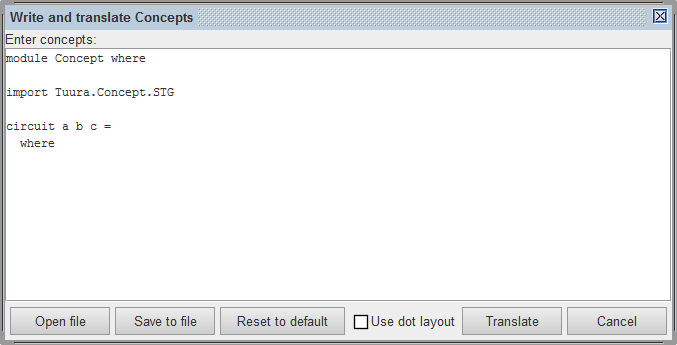
\includegraphics[scale=0.45]{Images/concepts_dialog_screenshot.png}
\par\end{centering}

\begin{centering}
\protect\caption{\label{fig:concepts_dialog_screenshot}The concepts dialog.}

\par\end{centering}
\vspace{-4mm}
\end{figure}

%\vspace{-3mm}

From within this dialog, one can write their own concepts, from the default 
template as shown in Figure~\ref{fig:concepts_dialog_screenshot}, or open an 
existing concepts file, with the \emph{.hs} extension. When satisfied with the 
concepts written, a user can choose to save the file, if not already saved, and
then translate these concepts.

\begin{figure}[h]
\begin{centering}
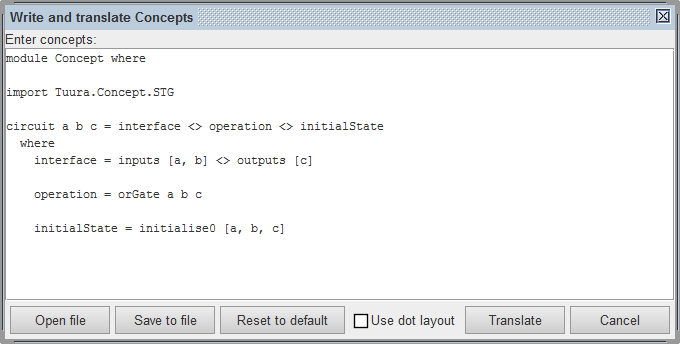
\includegraphics[scale=0.45]{Images/concepts_dialog_or_gate.png}
\par\end{centering}

\begin{centering}
\protect\caption{\label{fig:concepts_dialog_or_gate}The concepts dialog with a 
			specification typed in.}

\par\end{centering}
\end{figure}

Figure~\ref{fig:concepts_dialog_or_gate} is the concepts dialog after we have 
opened the OR-gate example concept specification 
(Section~\ref{sub:file_layout}). Clicking translate at this point will produce 
an STG representation of these concepts inthe workspace. 


\begin{figure}[h]
\begin{centering}
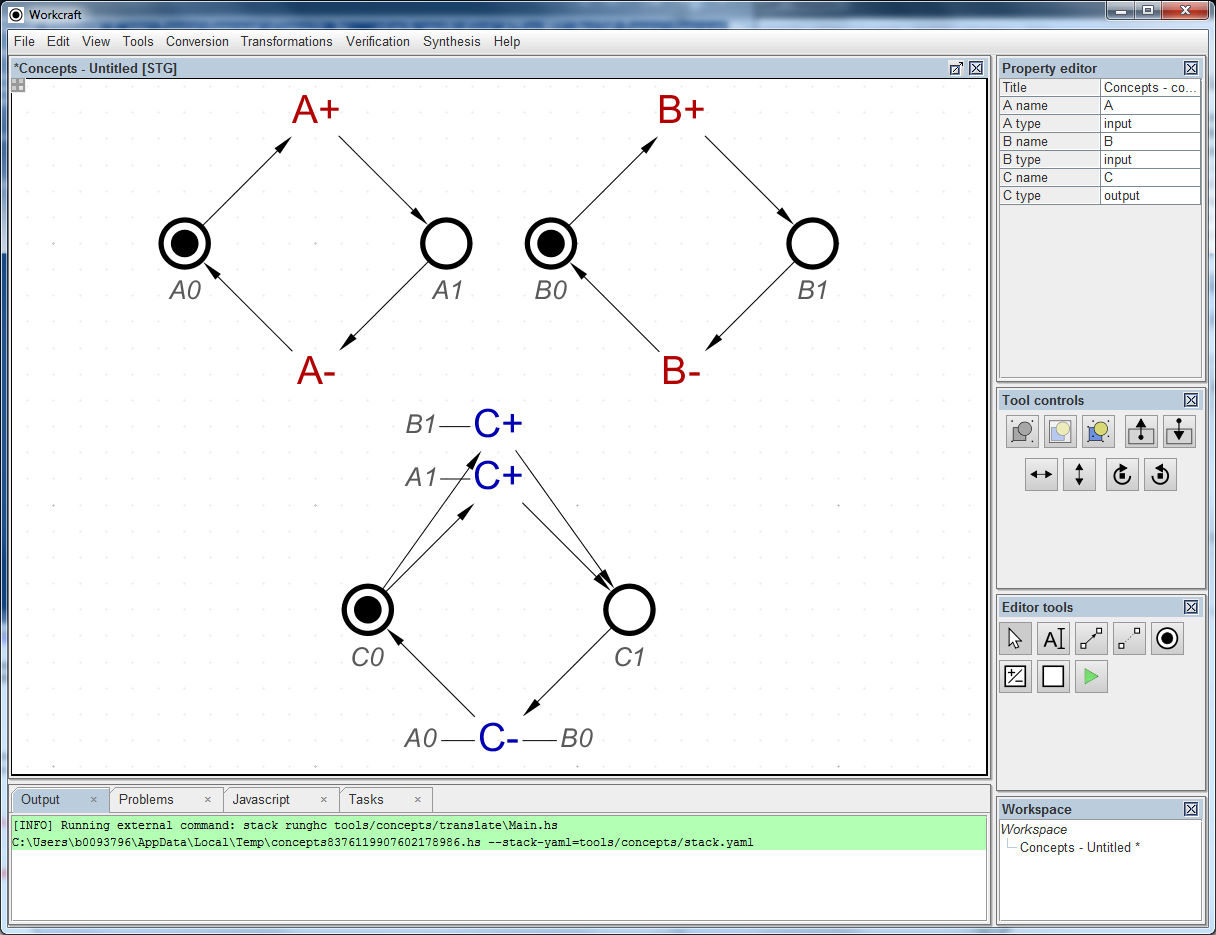
\includegraphics[scale=0.2]{Images/concepts_translated.png}
\par\end{centering}

\begin{centering}
\protect\caption{\label{fig:concepts_translated}The STG produced from 
			translating the concepts.}

\par\end{centering}
\vspace{-4mm}
\end{figure}



The translated concepts will look as shown in 
Figure~\ref{fig:concepts_translated}. Now, a user can choose to insert more 
concepts, make changes to this STG, and once they are satisfied with it, can 
then perform various functions on this STG. One can perform transformations, 
verifications, simulations and synthesis on this STG using the menus within this 
workspace. Any further changes to this STG, based on the results of these 
operations can be made to this STG or to the concepts file. 

\vspace{-3mm}

\subsection{Importing concepts directly}

\vspace{-2mm}

In \noun{Workcraft} it is also possible to import concepts directly from a file,
without having to view the concepts first. This can be done from the 
``\emph{File}'' menu, by selecting the ``\emph{Import...}'' option. 

\begin{figure}[H]
\begin{centering}
\vspace{-3mm}
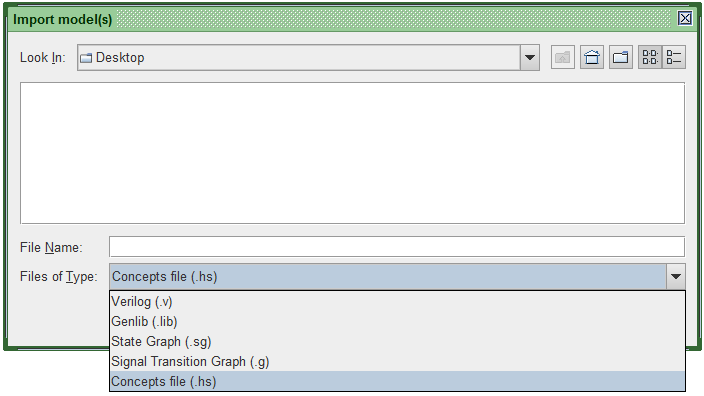
\includegraphics[scale=0.4]{Images/import_menu_screenshot.png}
\par\end{centering}

\begin{centering}
\protect\caption{\label{fig:import_menu_screenshot}The import menu and the 
			option of \emph{.hs} files.}

\par\end{centering}
\vspace{-3mm}
\end{figure}

When importing concepts using this menu, ensure to set the 
``\emph{Files of Type}'' option to ``\emph{Concepts file (.hs)}'', as shown in 
Figure~\ref{fig:import_menu_screenshot}. Any concept files imported will be
automatically translated to an STG.

\vspace{-3mm}

\subsection{Errors}

\vspace{-2mm}

If any errors are encountered during the translation process, \noun{Workcraft} 
will produce a helpful error message. This usually can tell you with more 
detail what the issue that is causing the error is, but will ask you to refer 
to \noun{Workcraft}'s console window for specific line numbers or signals which
need to be corrected. 

These errors will include whether a signal has not been declared as an input or
output, a signal has not had it's initial state given, or even that \noun{Plato}
has not been installed correctly. 

\vspace{-3mm}

\vspace{-2mm}

\section{Conclusions and future work\label{sec:conclusions}}

\vspace{-3mm}

In this work, we have displayed the process of specifying behavioural and 
compositional concepts for asynchronous circuits, using an open-source
tool, \noun{Plato}~\cite{2016_concepts_github}. This tool implements a domain-specific 
language, featuring some built-in concepts at varying levels, allowing users to
specify behaviours in a preferred way. 

This tool also features translation, a method of converting concepts into Signal
Transition Graphs, output in a format usable by other existing design, 
verification and synthesis tools. 

\noun{Plato}, can be used on it's own using a command-line interface, and is
integrated into \noun{Workcraft}, which can visualise many graphical modelling
methods, including STG which can be automatically imported from the
tool, either from concept specifications written by a user from within 
\noun{Workcraft}, or by importing a previously written concept file.
\noun{Workcraft} also features several verification and synthesis tools 
integrated, which can automatically use STGs translated from concepts. 

Using concepts, a user can reduce the time of designing an asynchronous
control circuit from the ground up, as well as allow reuse of components
either as part of a scenario or entire scenarios to reduce the design-time
of future projects. Composition of concepts can help
reduce errors and save time in comparison to performing these manually.
This method can help to make asynchronous circuits more appealing
to industrial designers.

Currently, this method works with Signal Transition Graphs, however
it can be applied to other modelling disciplines, such as Finite State
Machines~(FSM), and an automated concepts to FSM translation method
is aimed to be implemented.

%\emph{Process mining} can also be used for various purposes in conjunction
%with designing asynchronous circuits. For example, process mining can discover
%a behavioural model when none currently exists, and can be used to check 
%that an existing specification is realistic, or find less complex models. 
%All of this can be performed automatically, by tools such as
%\noun{PGminer}~\cite{mokhov2016mining}, given
%an event log with observations of a real analogue or digital system, and aid a
%designer in reducing design time and errors. We aim to test the possibility of 
%producing concepts directly from the mining of these event logs.

The \noun{Plato} tool we have discussed is available 
from~\cite{2016_concepts_github}, and as stated, is integrated into 
\noun{Workcraft}~\cite{Workcraft_website}. A manual is included with the tool, 
which features descriptions of the features. We host a regularly updated blog 
which discusses some interesting properties of concepts, and new ideas we find 
for concepts, and this is available  at~\cite{2016_blog_concepts}.

%\vspace{-2mm}

\bibliographystyle{unsrt}
\bibliography{publications}

\end{document}
